\graphicspath{{chapters/chapter4/img/}}

\chapter{Results and discussion}
\label{cha:results}

This chapter is meant to show and discuss the results obtained from the application of the methods introduced in \Cref{cha:methods}. The following graphics display in the majority of the case only a subset of emotions (i.e. anger, joy, fear, and sadness) for better data visualization.

\begin{figure}[H]
	\centering
    	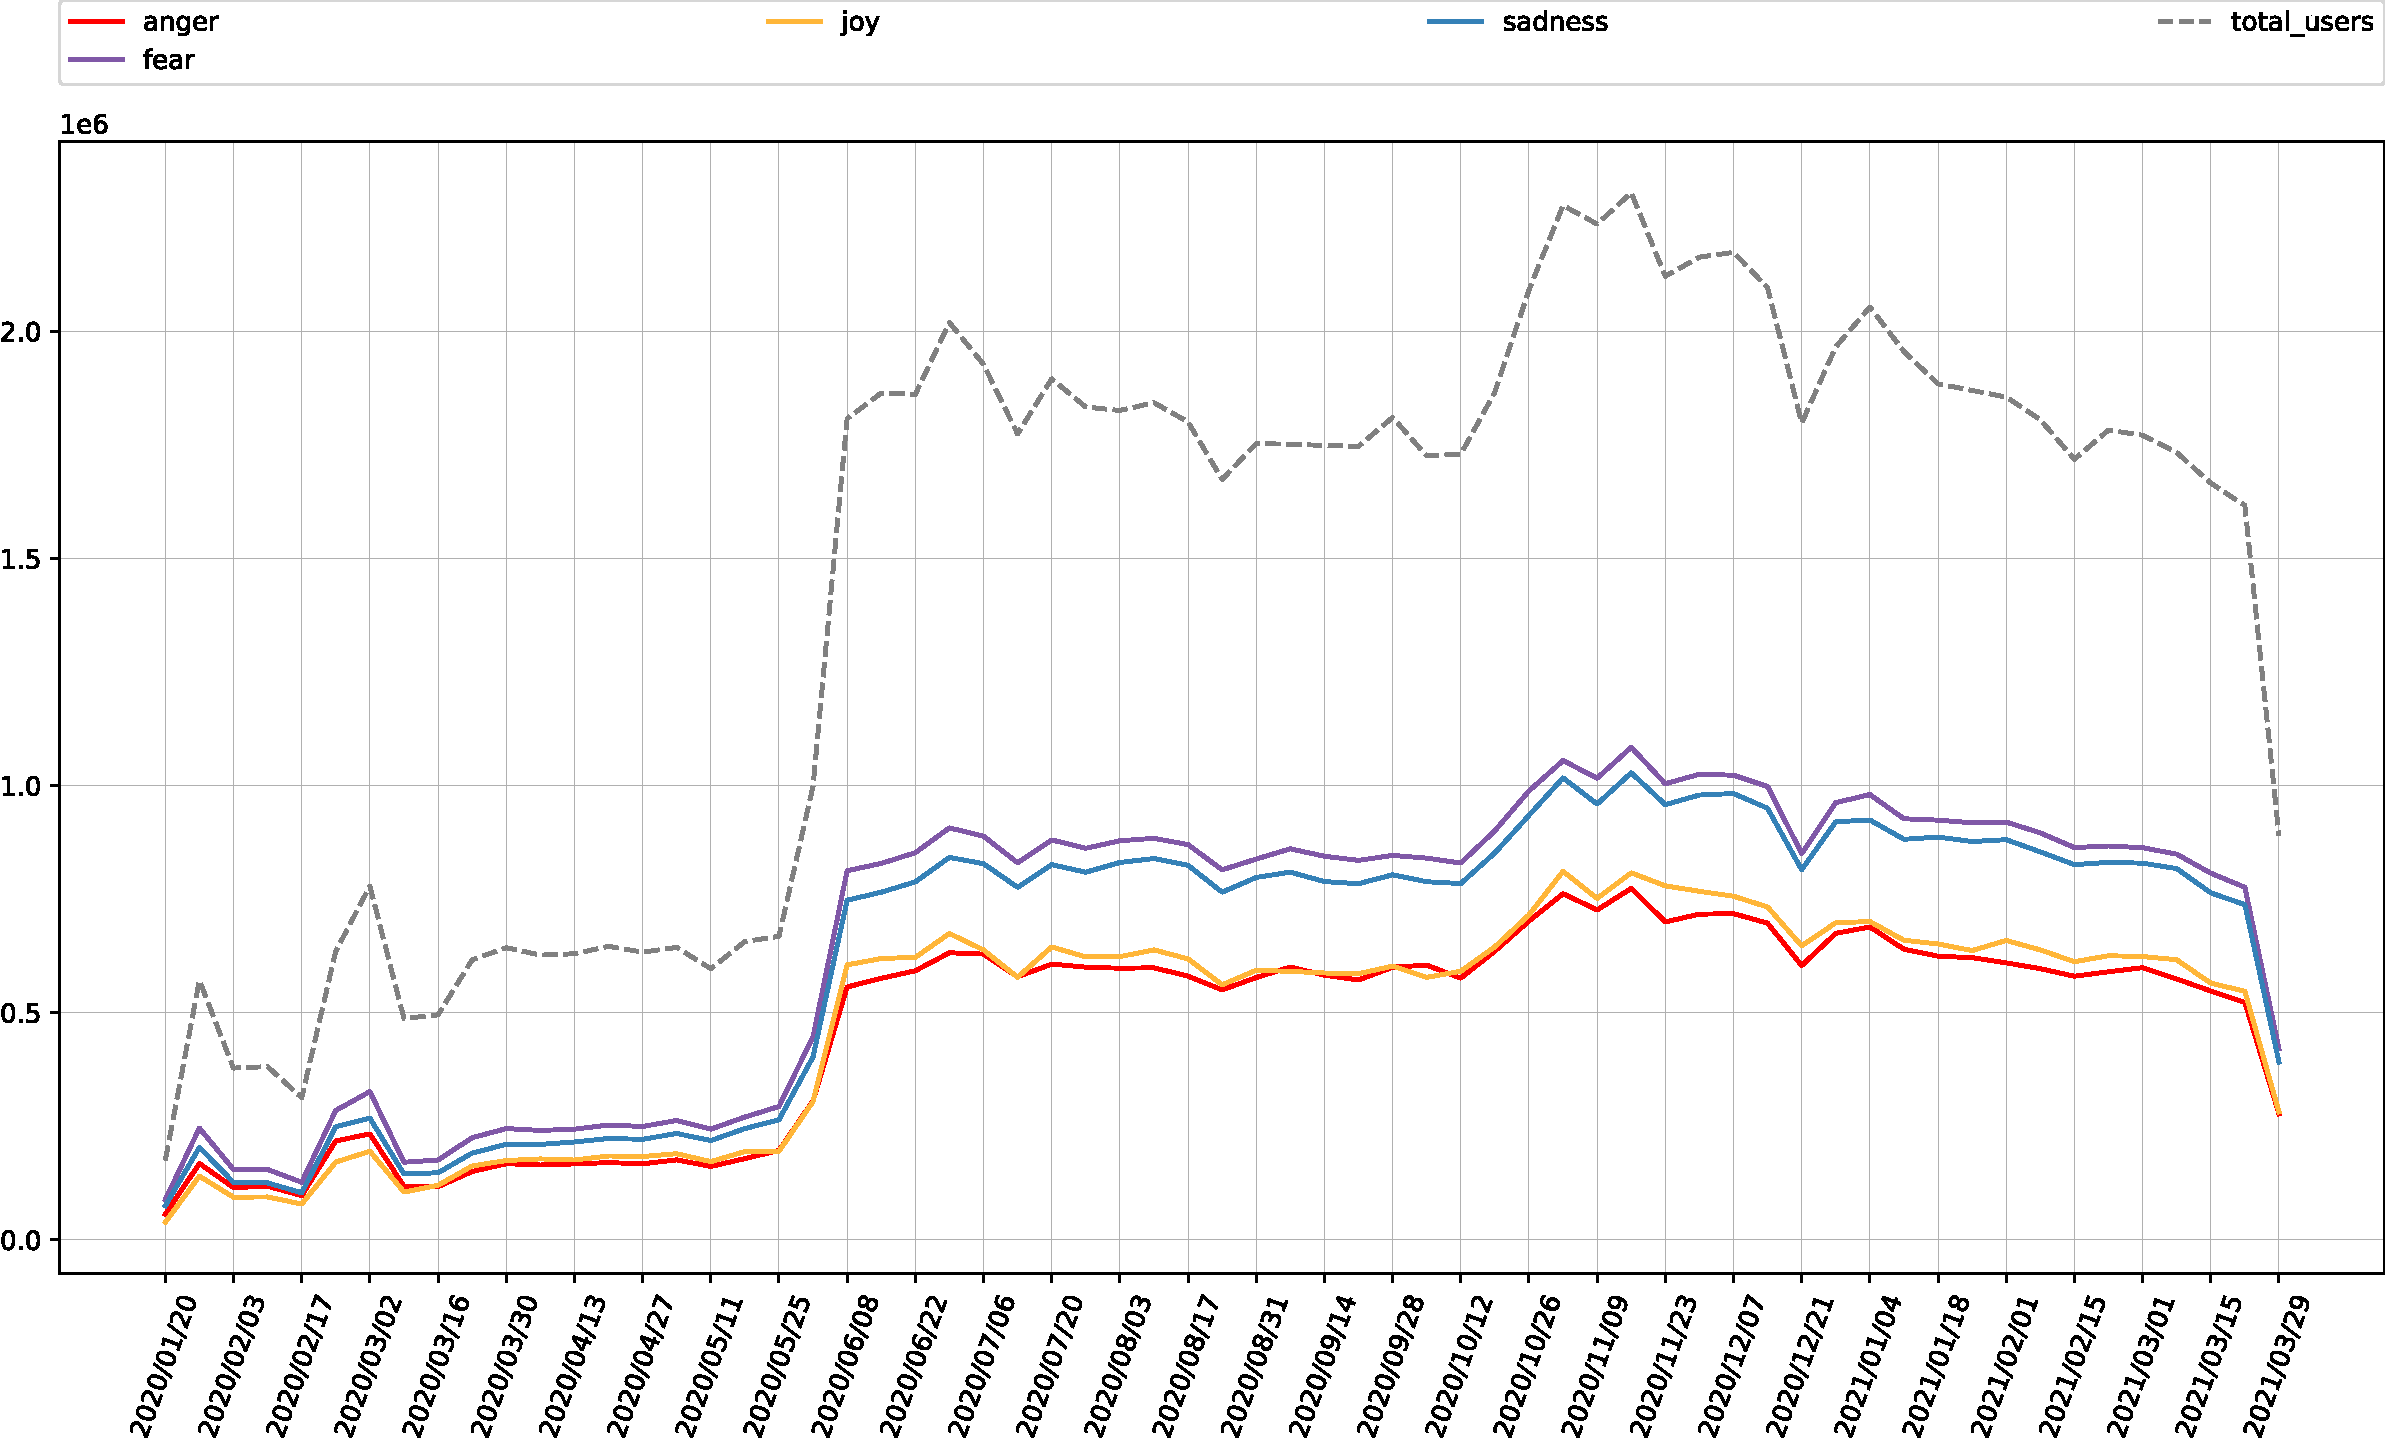
\includegraphics[scale=.35]{en_4_emotions_abs.svg}
    	\caption{Number of weekly users per emotion for the English tweets}
    	\label{fig:en-4-emotions-abs}
\end{figure}

\Cref{fig:en-4-emotions-abs} displays the number of users that expressed a particular emotion in a given week, considering the English tweets. Instead, the gray dashed line indicates the number of users that posted at least one tweet during a week. The fact that the data collection migrated to AWS around June 2020, explains why the number of tweets almost doubled from 01/06/2020 to 08/06/2020.

\begin{figure}[H]
	\centering
    	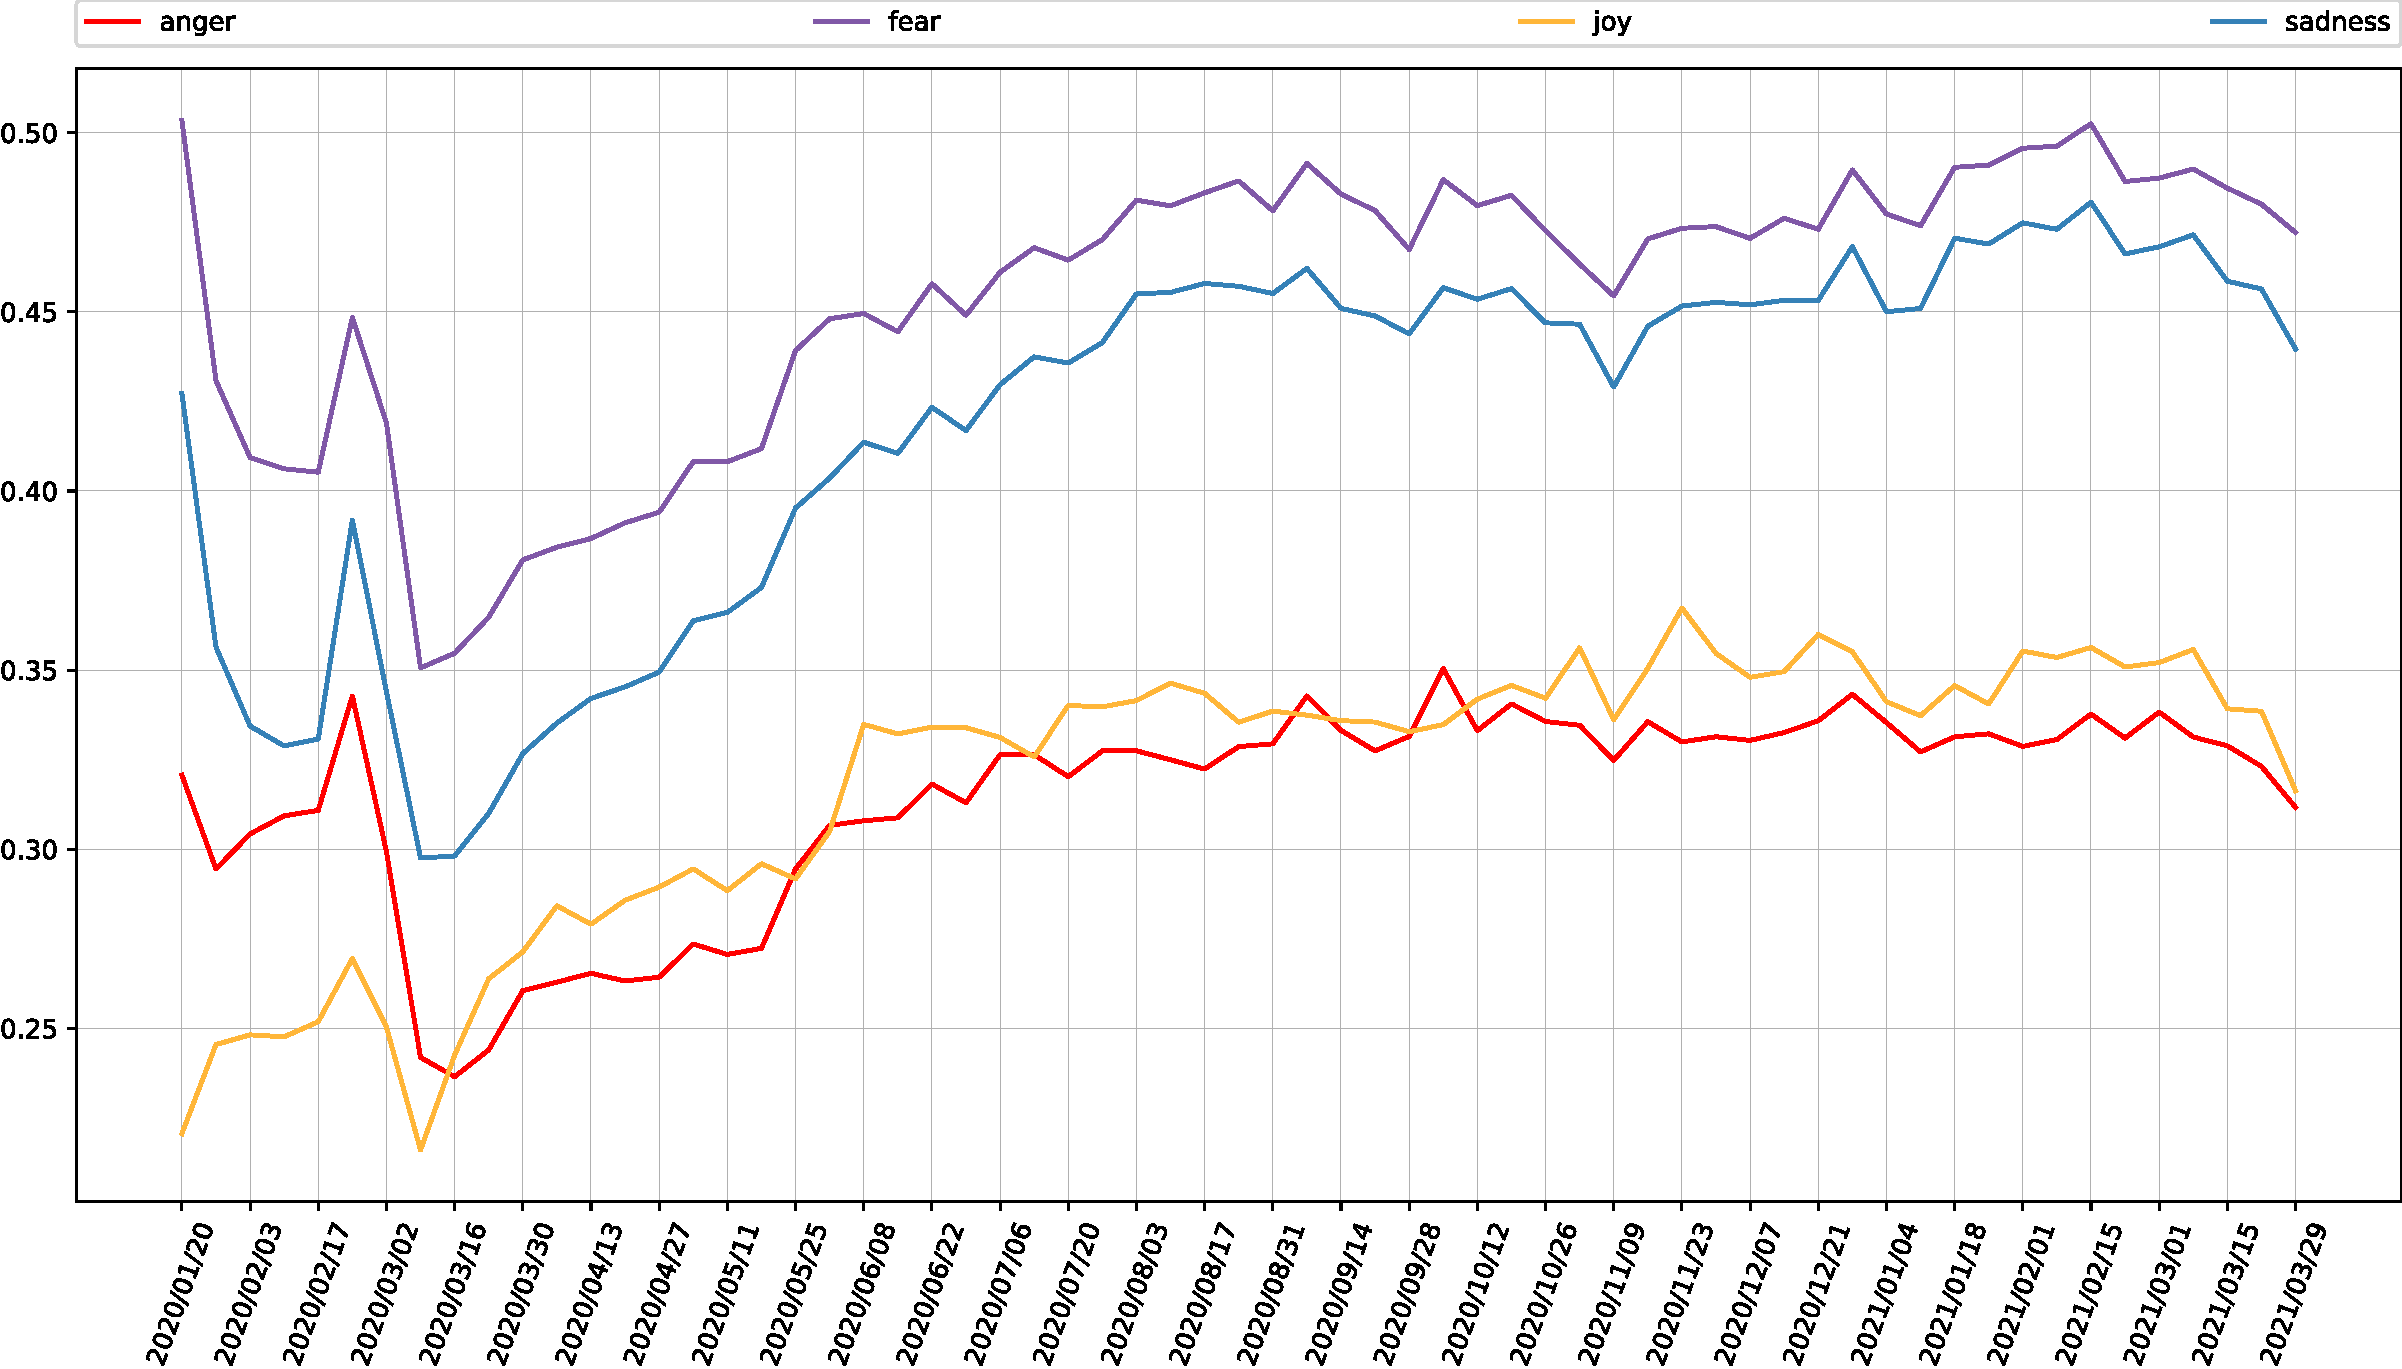
\includegraphics[scale=.35]{en_4_emotions.svg}
    	\caption{Proportion of weekly users per emotion for the English tweets}
    	\label{fig:en-4-emotions}
\end{figure}

\Cref{fig:en-4-emotions} instead shows the proportion of users that expressed a particular emotion in a given week considering in the English tweets. Here we can notice some interesting results: first of all, there are some cases where all the emotions seem to have the same courses. We would have expected that, if negative emotions increased, positive emotions would decrease (and vice versa). Instead, during the week starting from 24/02/2020, the proportion of users that expressed anger, joy, fear, and sadness raised. This probably happened because users during that time were particularly emotional and used several more words within a tweet. However, that is not always the case: for example, during 13/07/2020 the joy decreased, while fear, and sadness increased.

Secondly, it is also possible to observe how time frames of greater joy alternate with periods of greater anger. However, this is not the case for example of fear and sadness. This probably happens because there are a lot of words that convey both these emotions at the same time. In practice, when one increases, so does the other.

\begin{figure}[H]
	\centering
    	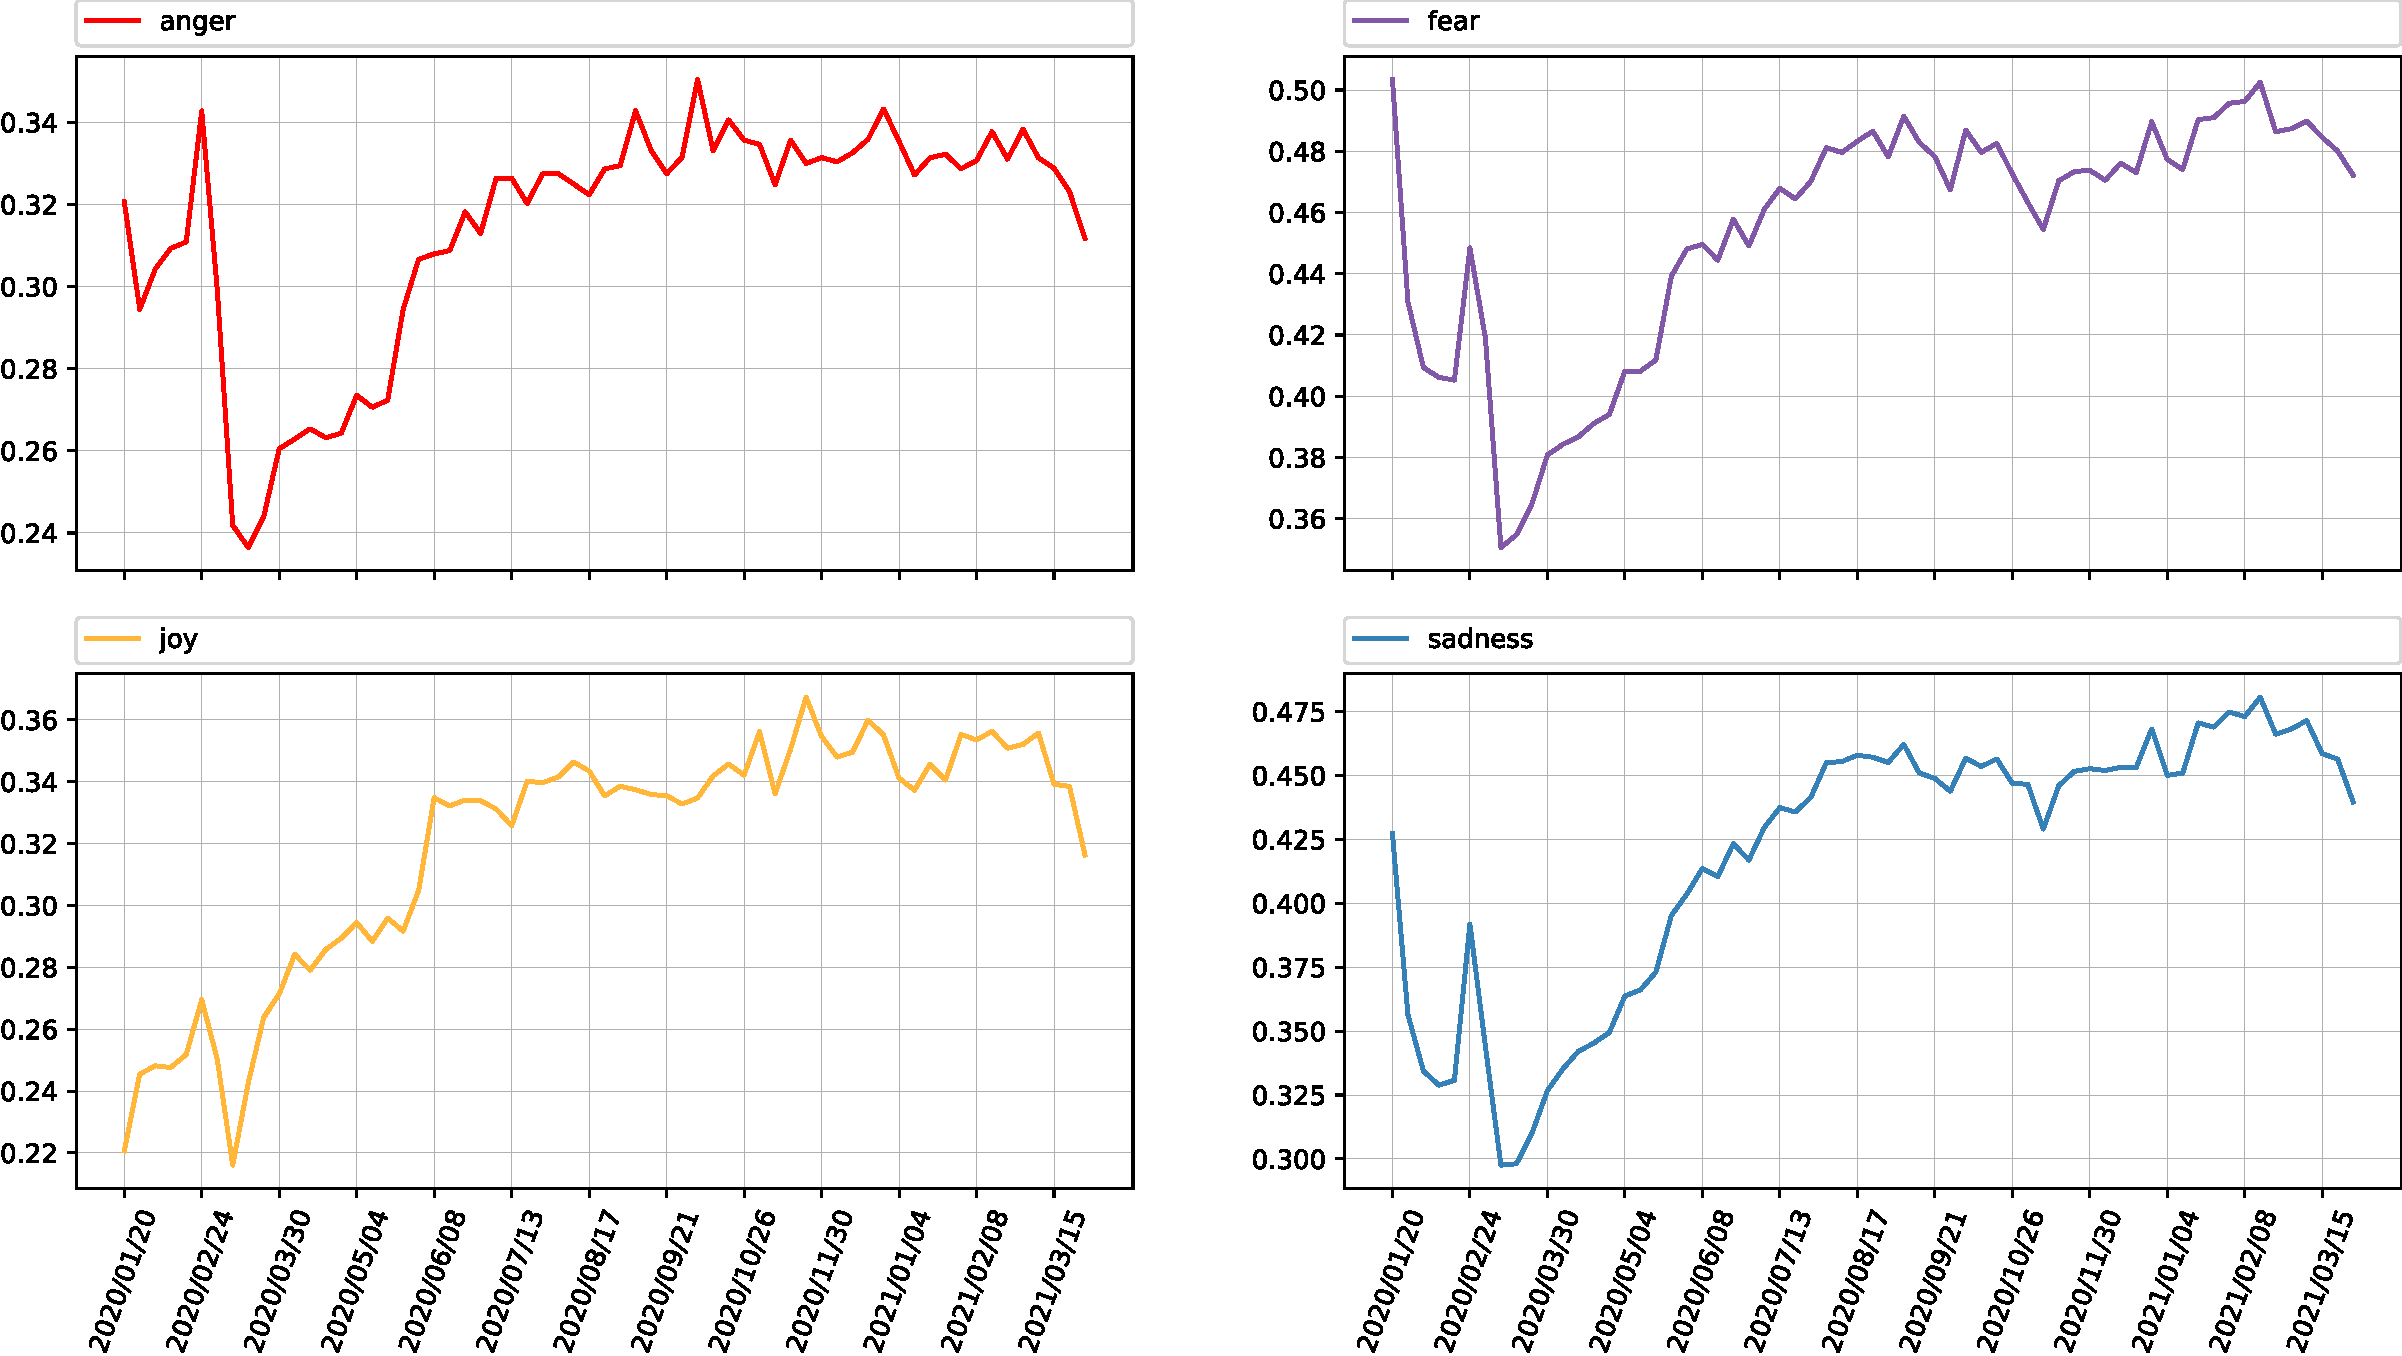
\includegraphics[scale=.35]{en_4_emotions_subplot_1.svg}
    	\caption{Proportion of weekly users expressing a particular emotion for the English tweets (subplots)}
    	\label{fig:en-4-emotions-subplot-1}
\end{figure}

Before approaching the data normalization, we have also tried to divide the different emotions courses into subplots. If we take a look at \Cref{fig:en-4-emotions-subplot-1}, both global (and local) maxima and minima are visible to the naked eye. However, the comparison between different emotions becomes really difficult.

\begin{figure}[H]
	\centering
    	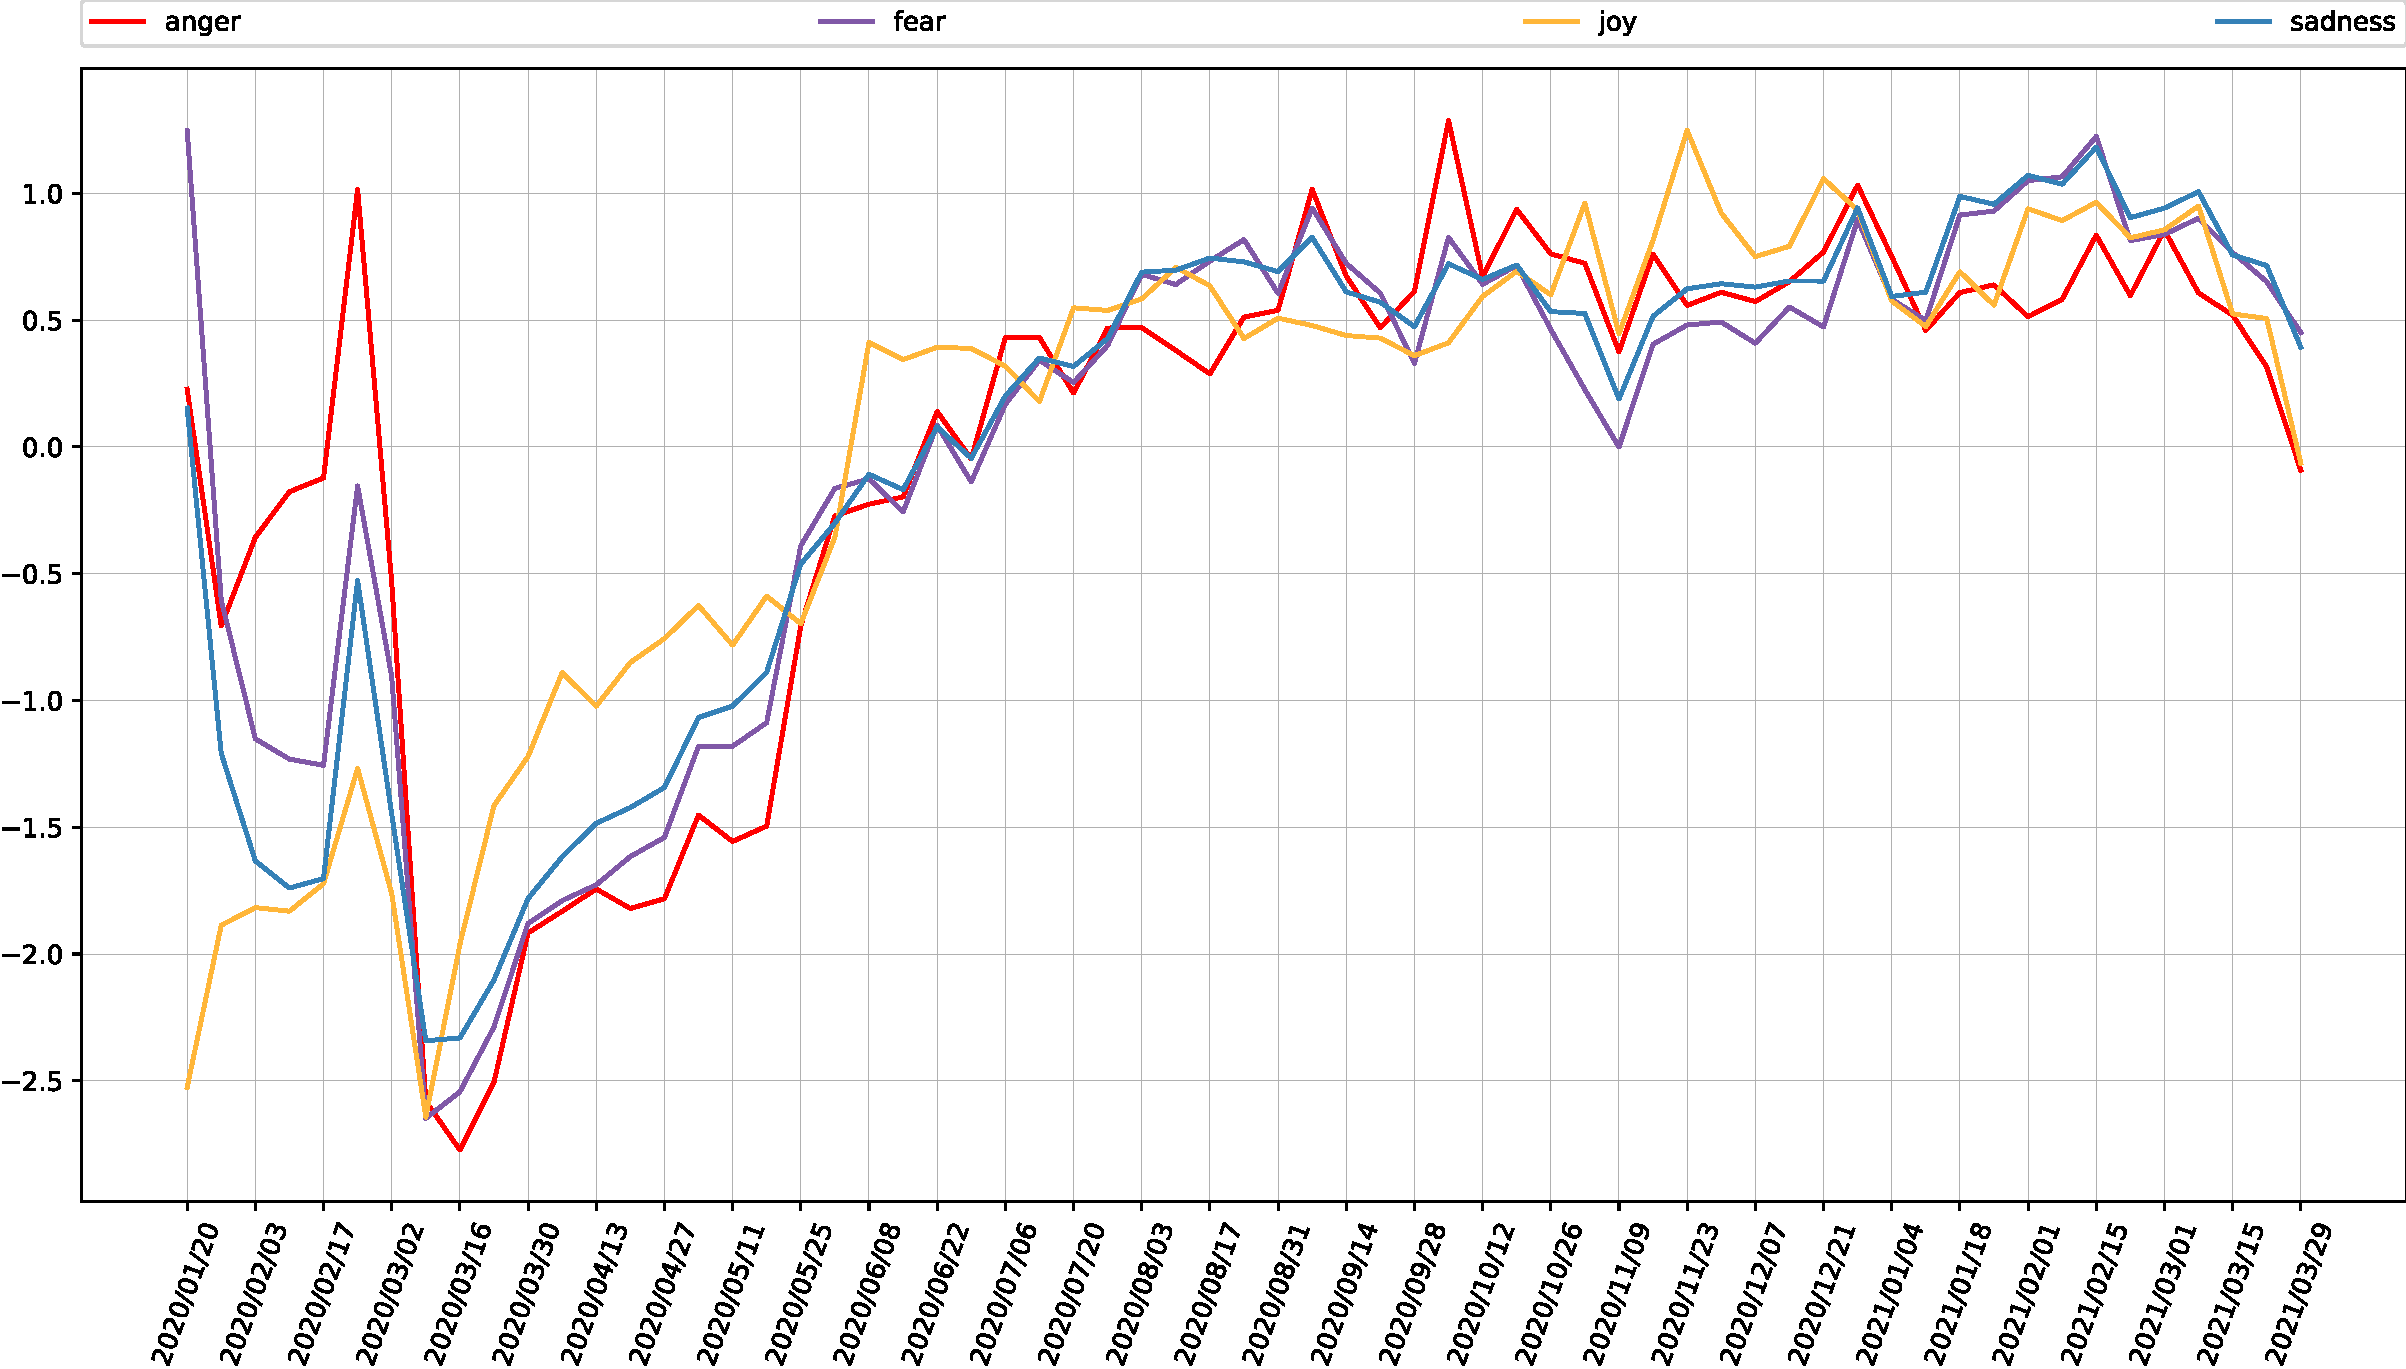
\includegraphics[scale=.35]{en_4_emotions_standardized.svg}
    	\caption{Z-score of weekly users per emotion for the English tweets}
    	\label{fig:en-4-emotions-std}
\end{figure}

The z-score instead proved to be a very useful data normalization. As we can see from \Cref{fig:en-4-emotions-std}, not only peaks are noticeable even if we are considering the emotions altogether, but we can also understand which time frames were characterized by a greater (or lower) emotion value w.r.t. the mean value of that particular emotion. For example, it is possible to see that, starting from 16/03/2020, the proportion of users that expressed joy w.r.t. the mean value of joy over the whole period surpassed all the other emotions w.r.t. their mean value over the whole period. 

\begin{figure}[H]
	\centering
    	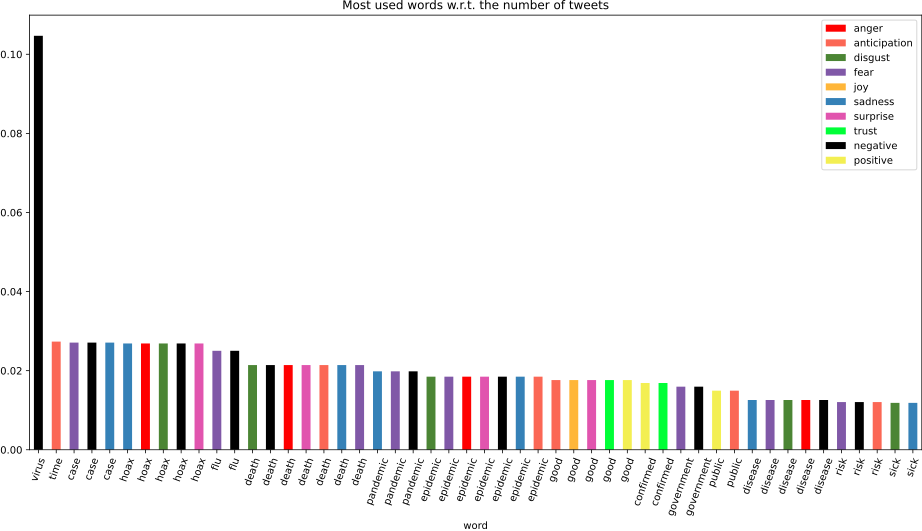
\includegraphics[scale=.35]{en_most_used_words_2020_02_24.svg}
    	\caption{Z-score of weekly users per emotion for the English tweets}
    	\label{fig:en-most-used-word-2020-02-24}
\end{figure}

\begin{figure}[H]
	\centering
    	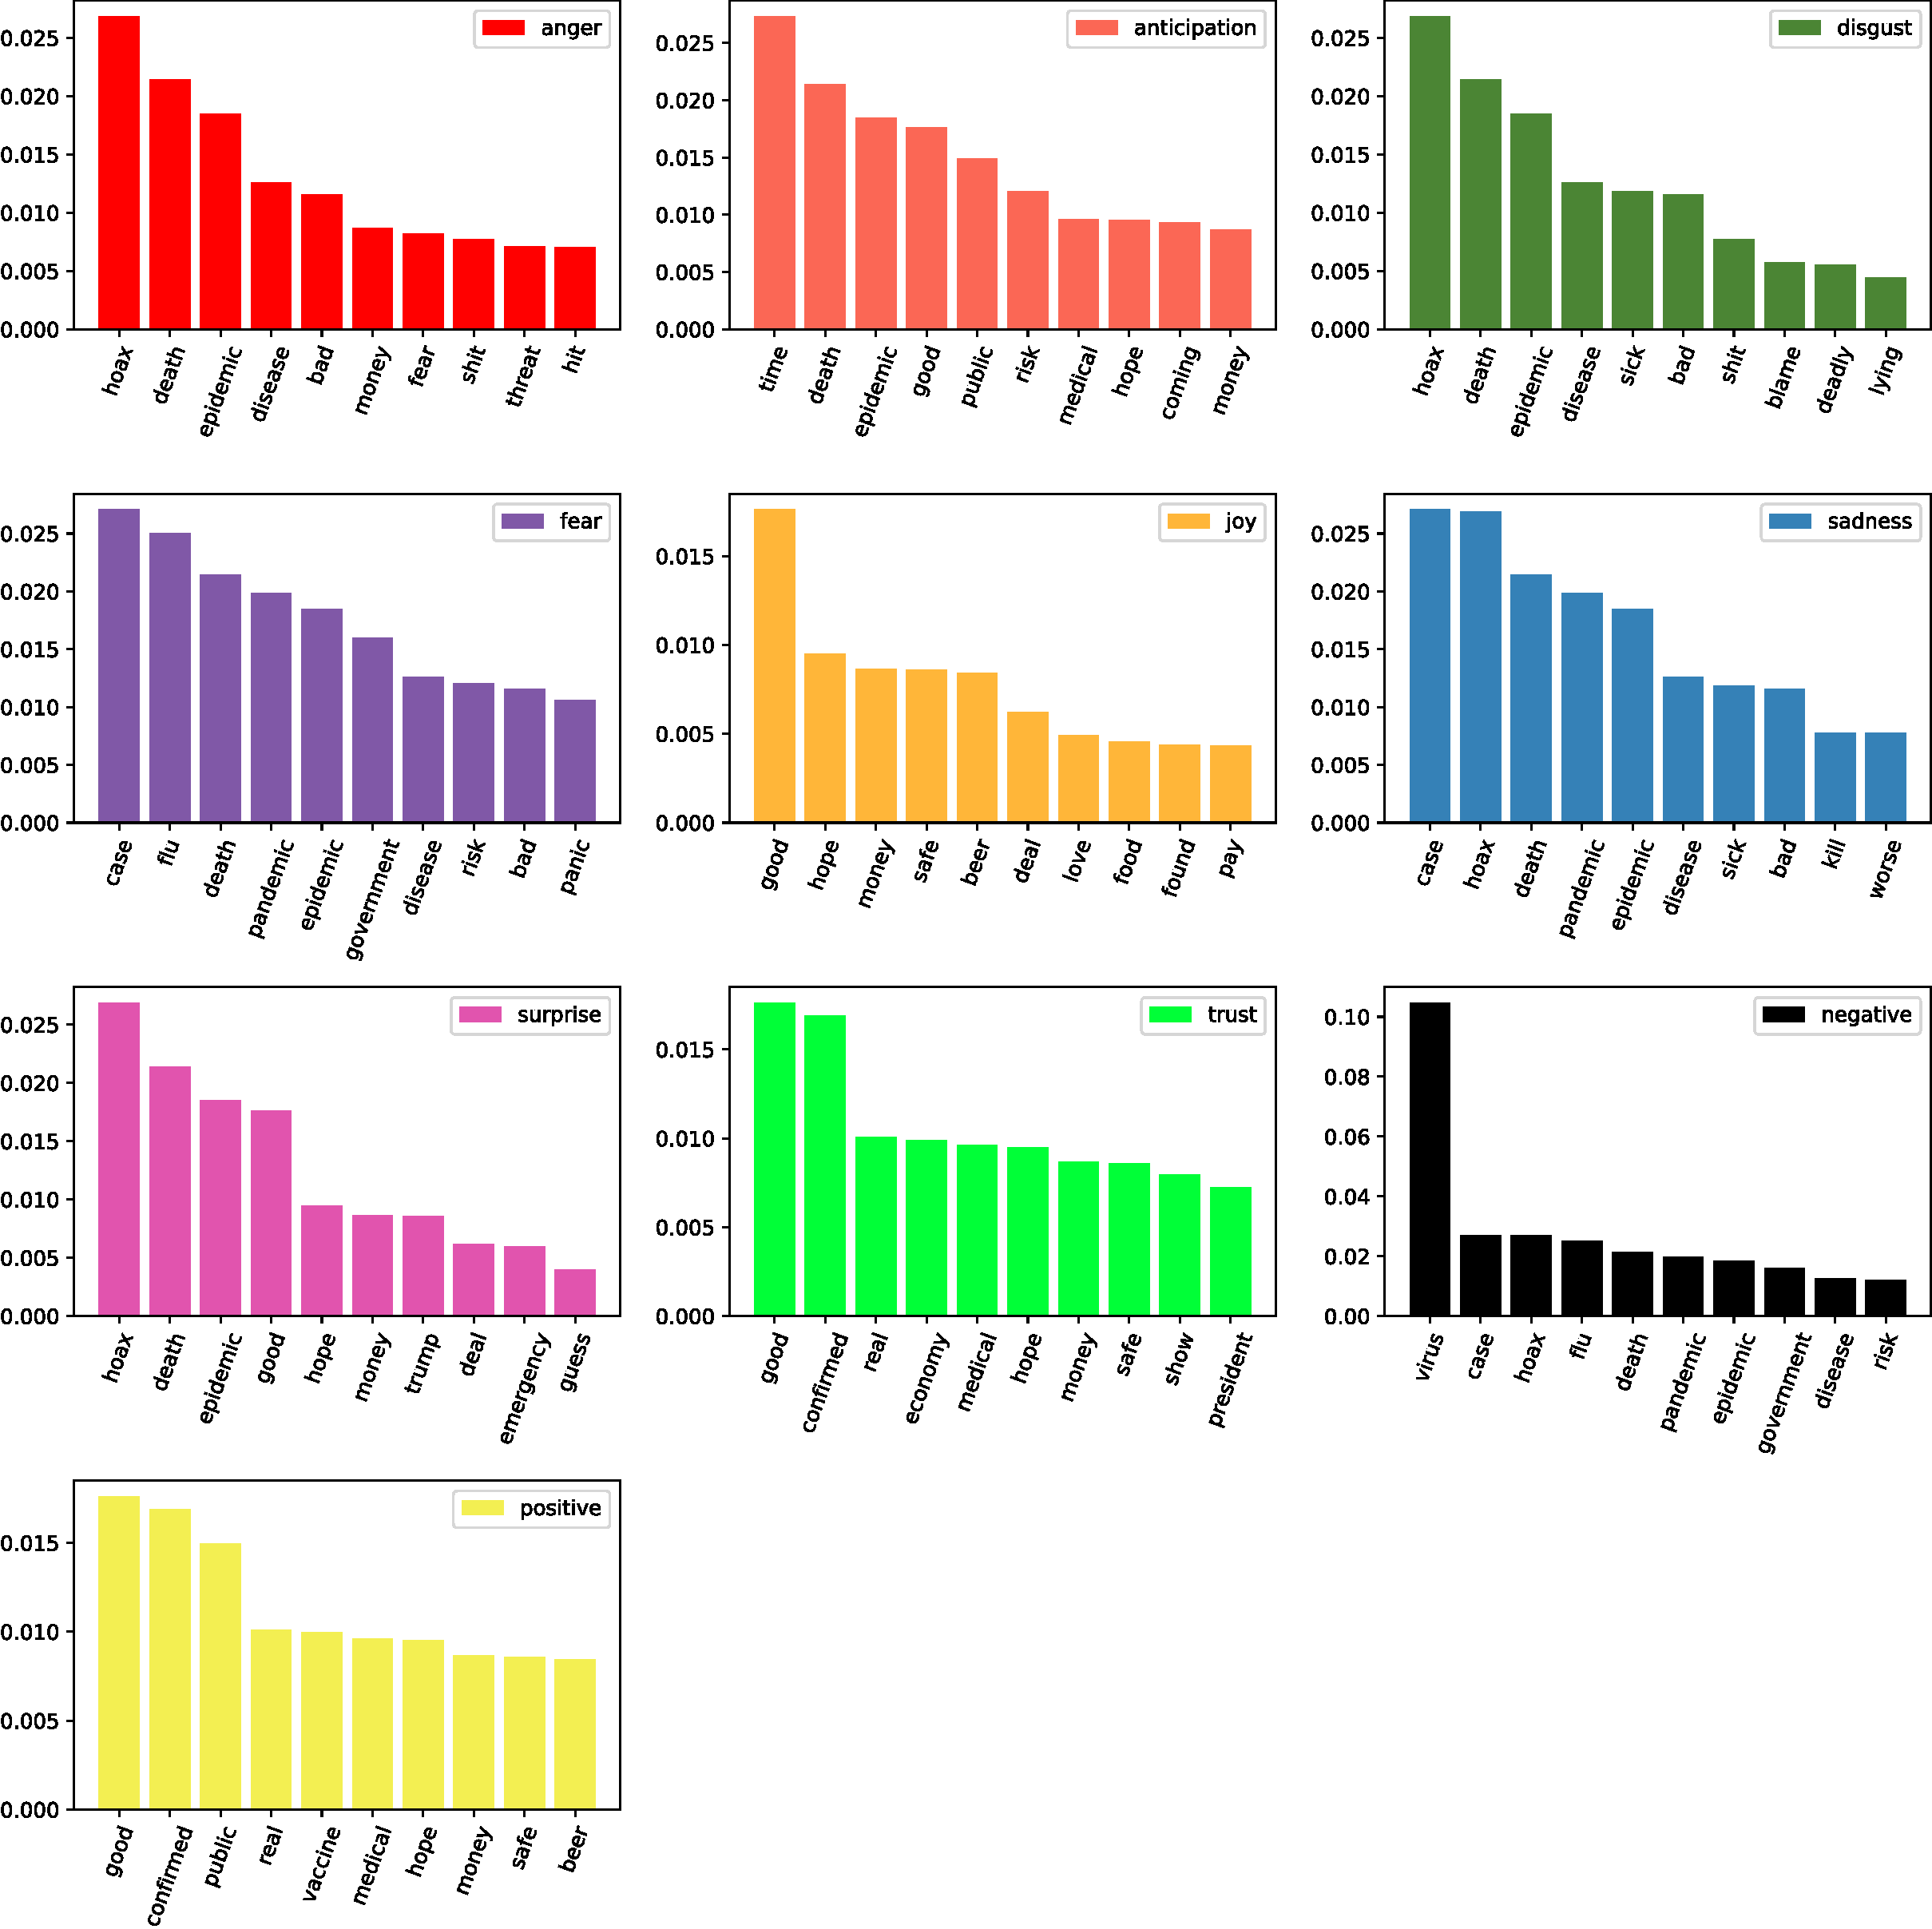
\includegraphics[scale=.35]{en_most_used_words_2020_02_24_subplot.svg}
    	\caption{Z-score of weekly users per emotion for the English tweets}
    	\label{fig:en-most-used-word-subplot-2020-02-24}
\end{figure}

\begin{figure}[H]
	\centering
    	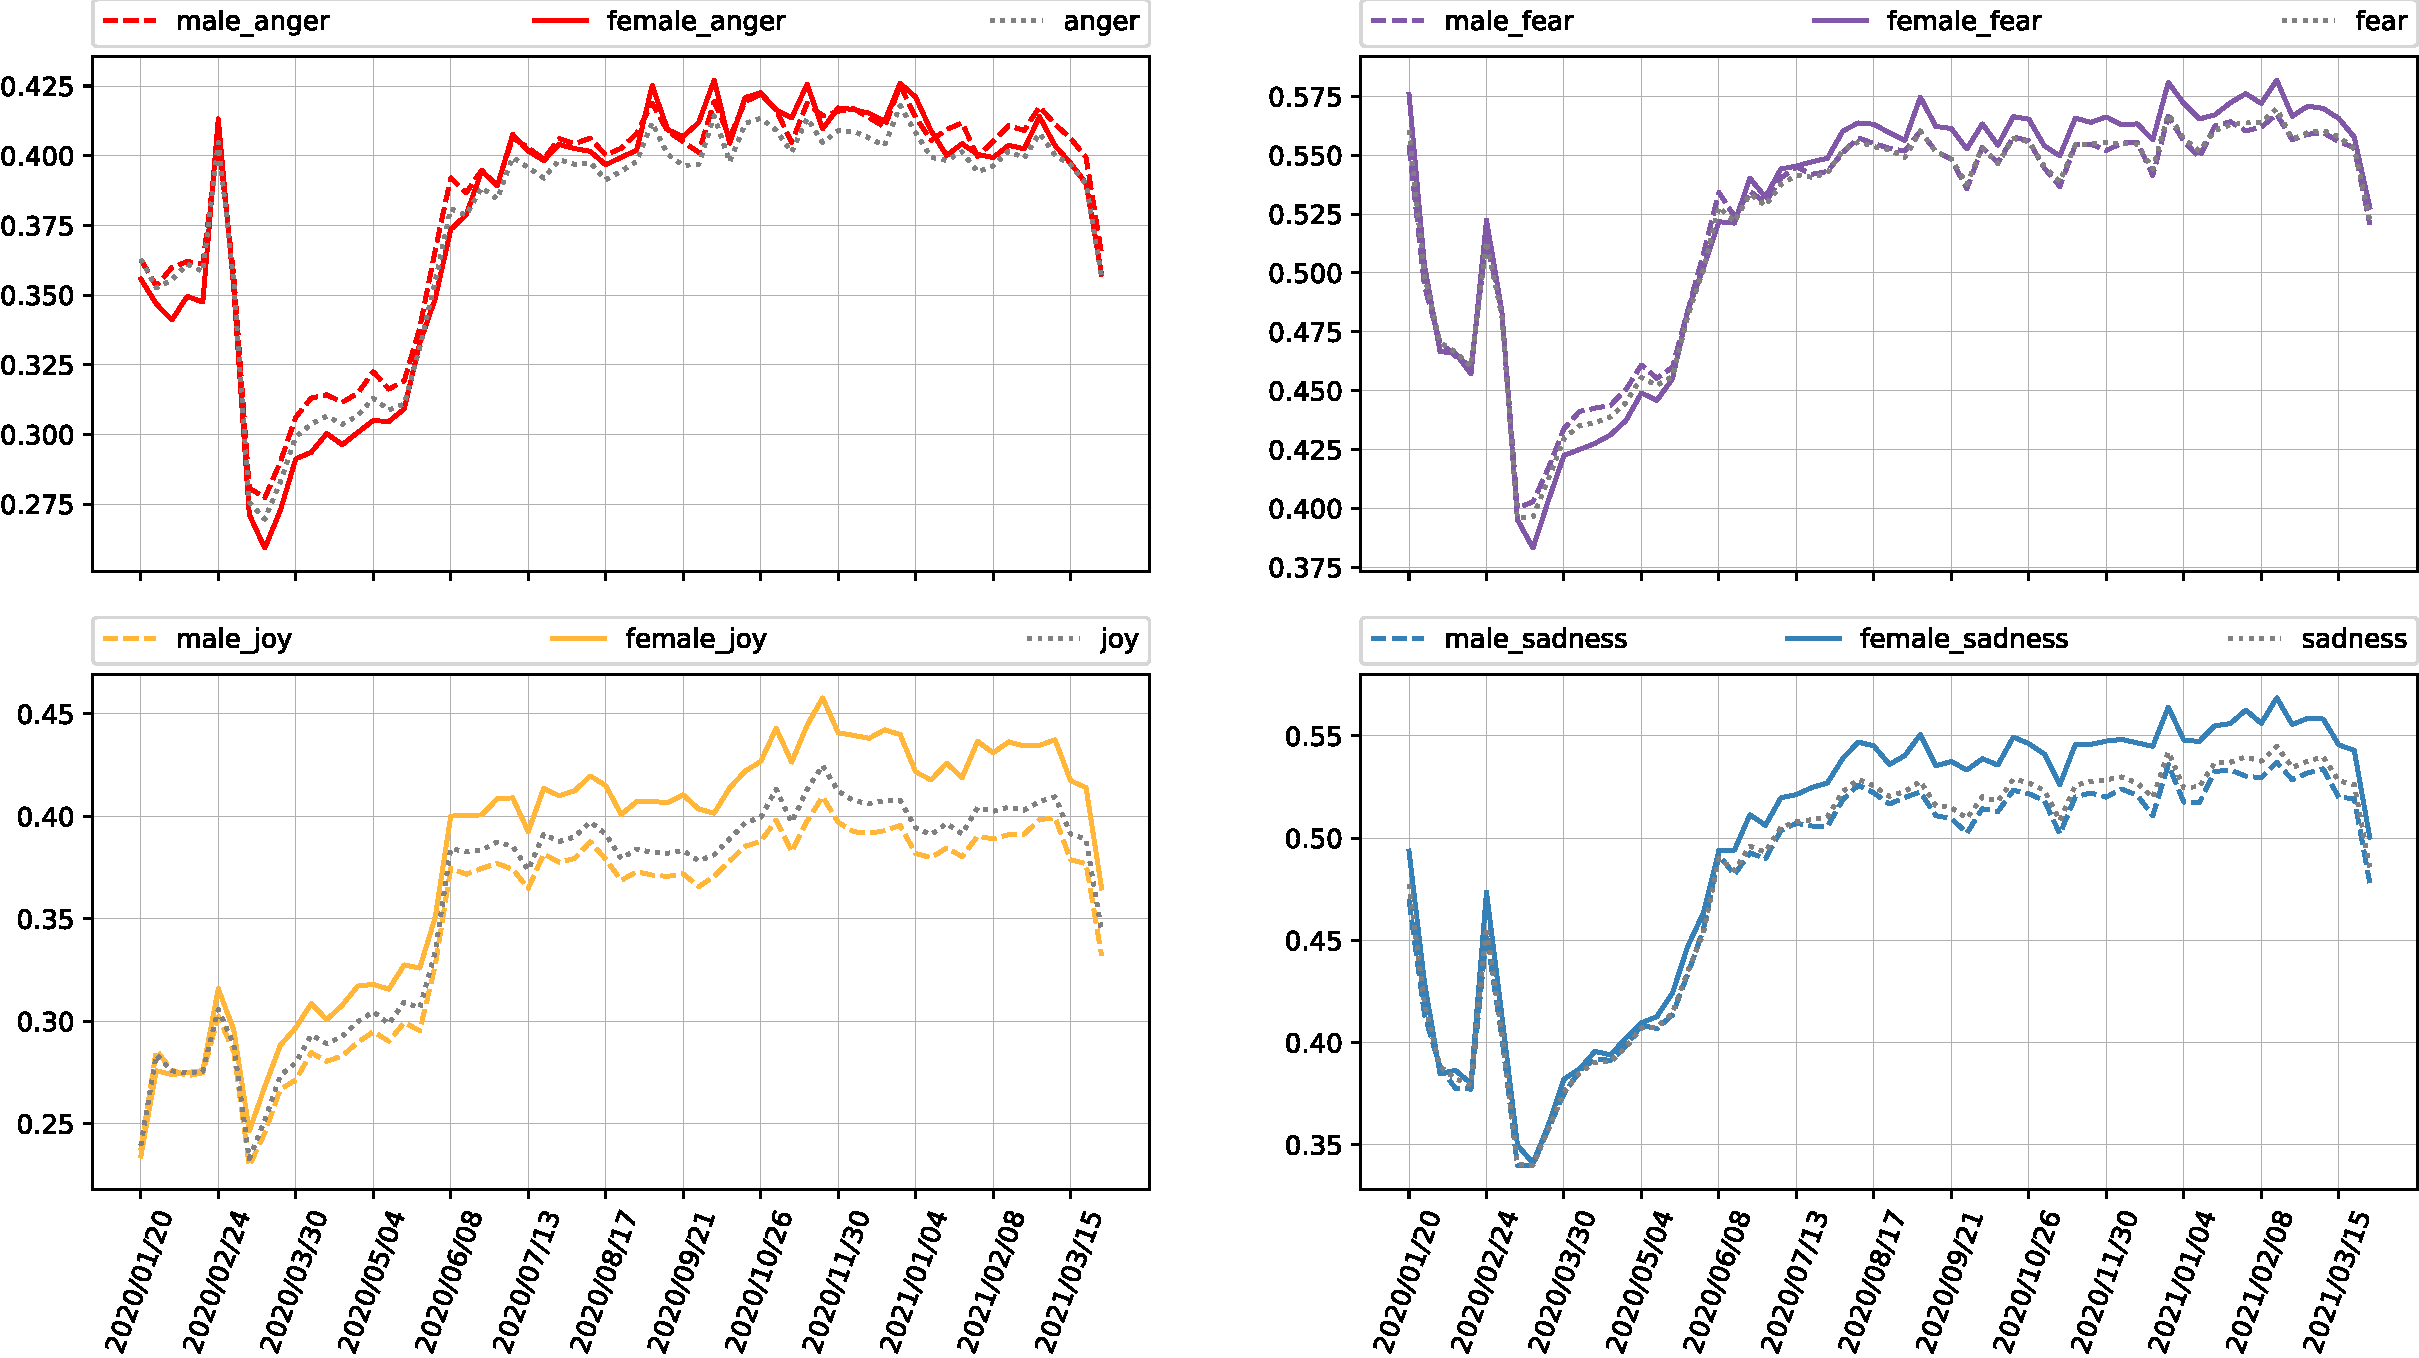
\includegraphics[scale=.35]{en_4_emotions_per_category_with_course_subplot_1.svg}
    	\caption{Z-score of weekly users per emotion for the English tweets}
    	\label{fig:en-4-emotions-per-category-course-subplot-1}
\end{figure}

\begin{figure}[H]
	\centering
    	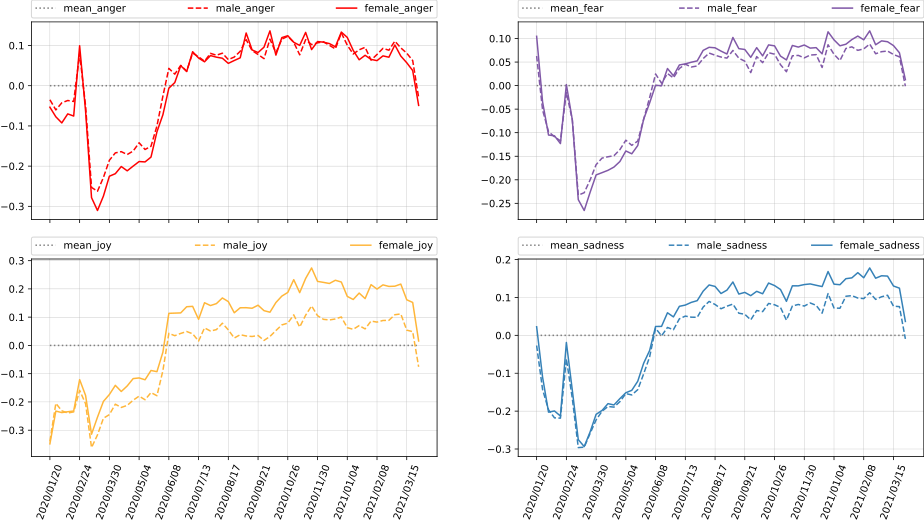
\includegraphics[scale=.35]{en_4_emotions_per_category_over_mean_subplot_1.svg}
    	\caption{Z-score of weekly users per emotion for the English tweets}
    	\label{fig:en-4-emotions-per-category-course-mean-1}
\end{figure}